%!TEX root = ../../presentation.tex

\begin{frame}[plain]{\hbox{Example Scenario: Punktförmige Zugbeeinflussung}}
  \textwidthplain
  \begin{tikzpicture}
    \node (tracks) {\includegraphics[width=10cm]{content/chapter_hardware_srv/pzb}};
    \path (tracks.south west)
      ++(0,-3mm) node[coordinate] (start) {}
      ++(9.5mm,0) node[coordinate] (vor) {}
        node[below=3pt] {250}
        node[above=1.8cm,text width=1cm,align=center] {distant\\signal}
      ++(5.85cm,0) node[coordinate] (magnet) {}
        node[below=3pt] {1000}
        node[above=1.8cm,text width=3cm,align=center] {500-Hz\\speed limiter}
      ++(1.93cm,0) node[coordinate] (haupt) {}
        node[below=3pt] {1250}
        node[above=1.8cm,text width=1cm,align=center] {stop\\signal}
      ++(5mm,0) node[coordinate] (ende) {}
        node[right] {pos. [m]};
    \path[thick]
      (start) edge (vor)
      (vor) edge[|-] (magnet)
      (magnet) edge[|-] (haupt)
      (haupt) edge[|->] (ende);
  \end{tikzpicture}
\end{frame}

\newcommand{\exampleSetup}{
  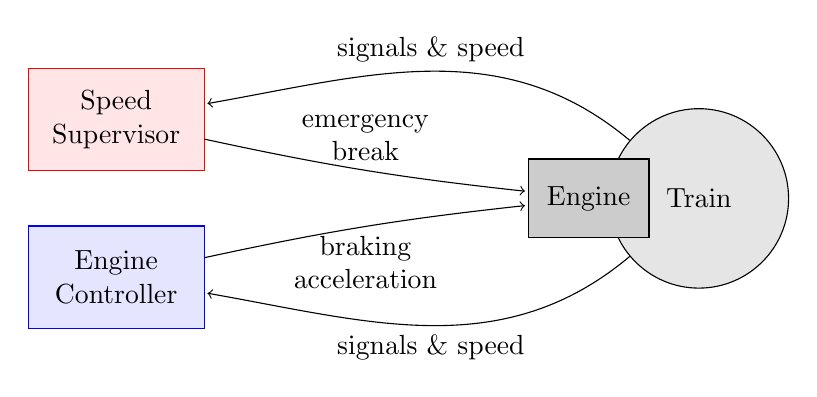
\begin{tikzpicture}[
    controller/.style={
      draw=blue,
      fill=blue!10,
      text width=2cm,
      minimum height=1.3cm,
      align=center
    },
    supervisor/.style={
      draw=red,
      fill=red!10,
      text width=2cm,
      minimum height=1.3cm,
      align=center
    },
    engine/.style={
      draw,
      fill=black!20,
      text width=1.3cm,
      minimum height=1cm,
      align=center
    },
    environment/.style={
      draw,
      circle,
      fill=black!10,
      text width=2cm,
      align=center
    }
  ]
    \node[supervisor] (supervisor) at (0,2) {Speed\\Supervisor};
    \node[controller] (controller) at (0,0) {Engine\\Controller};
    \node[environment] (environment) at (7.4,1) {Train};
    \node[engine] (engine) at (6,1) {Engine};

    \path[->, shorten >=1pt]
      (controller) edge[bend left=3] node[below] {\shortstack{braking\\acceleration}} (engine)
      (supervisor) edge[bend right=3] node[above] {\shortstack{emergency\\break}} (engine)
      (environment) edge[out=-140, in=-10] node[below] {signals \& speed} (controller)
                    edge[out=140, in=10] node[above] {signals \& speed} (supervisor);
  \end{tikzpicture}
}

\begin{frame}{Example Scenario: Braking a Train}
  \centering
  \exampleSetup
\end{frame}

\begin{frame}[t]{Example Scenario}
  \vskip-6mm\hfill
  \scalebox{.5}{\exampleSetup}
  \vskip4mm

  \centering
  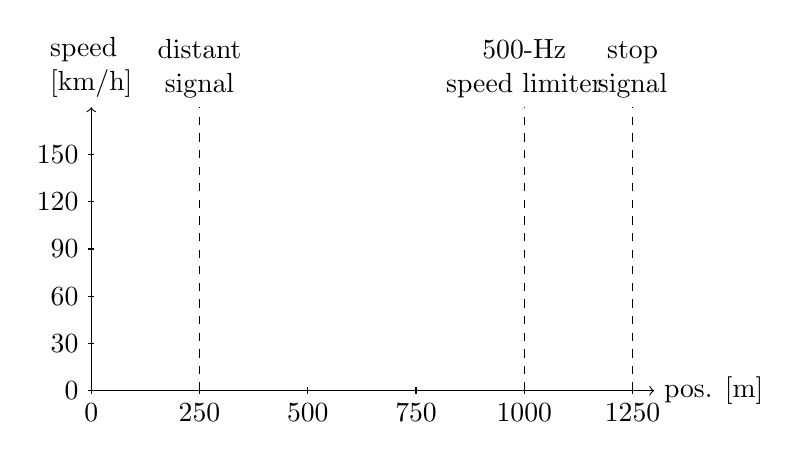
\begin{tikzpicture}[xscale=0.55,yscale=2]
    \foreach \x/\label in {2.5/distant\\signal,10/500-Hz\\speed limiter,12.5/stop\\signal} {
      \draw[dashed] (\x,0) -- (\x,1.8) node[above,text width=2cm,align=center] {\label} ;
    }
    \draw[red] plot file {content/chapter_hardware_srv/allowed_speed.table};
    \draw[blue] plot file {content/chapter_hardware_srv/speed.table};
    \draw[->] (0,0) -- (13,0) node[right] {pos. [m]};
    \draw[->] (0,0) -- (0,1.8) node[above] {\shortstack[l]{speed\\{[km/h]}}};
    \foreach \y/\label in {0/0,.3/30,.6/60,.9/90,1.2/120,1.5/150} {
      \draw (-2pt,\y) node[left] {\label} -- (2pt,\y);
    }
    \foreach \x/\label in {0/0,2.5/250,5/500,7.5/750,10/1000,12.5/1250} {
      \draw (\x,-.6pt) node[below] {\label} -- (\x,.6pt);
    }
  \end{tikzpicture}
\end{frame}